\documentclass[kravspec/krav.tex]{subfiles}

\begin{document}
\clearpage
\section{Kommunikationsmodul}
\begin{figure}[H]
    \centering
    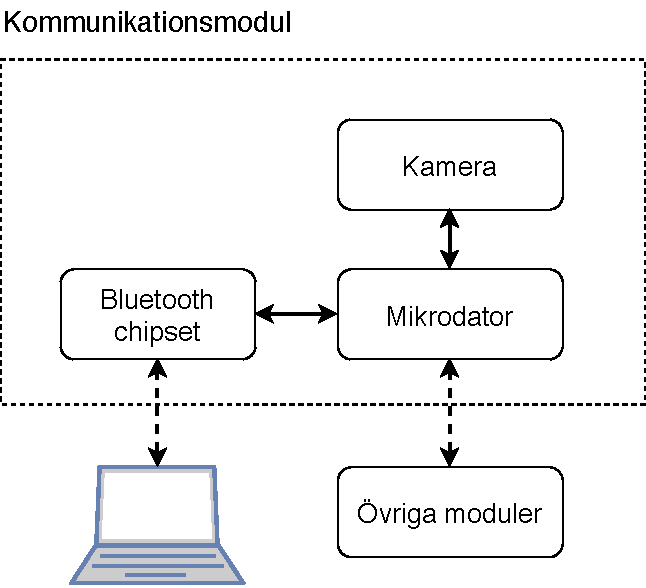
\includegraphics[width=0.6\linewidth]{kravspec/figures/kommunikationsmodul.pdf}
    \caption{Kommunikationsmodul}
    \label{fig:kommunikationsmodul}
\end{figure}
\subsection{Beskrivning}
Kommunikationsmodulen består av en mikrodator, ett bluetooth chipset samt en
kamera. Kommunikationsmodulen är huvudorganet i systemet och agerar som
dirigent. Dess uppgift består av bland annat bildbearbetning, dirigering av
information till andra moduler samt kommunikation med en dator.

Till datorn skickas positionen på bilen, avlagd sträcka, avstånd till
vägkant/hinder etc. Dessutom används datorn som kontroller vid manuell körning
av bilen.

\clearpage
\section{Styrmodul}
\begin{figure}[h]
    \centering
    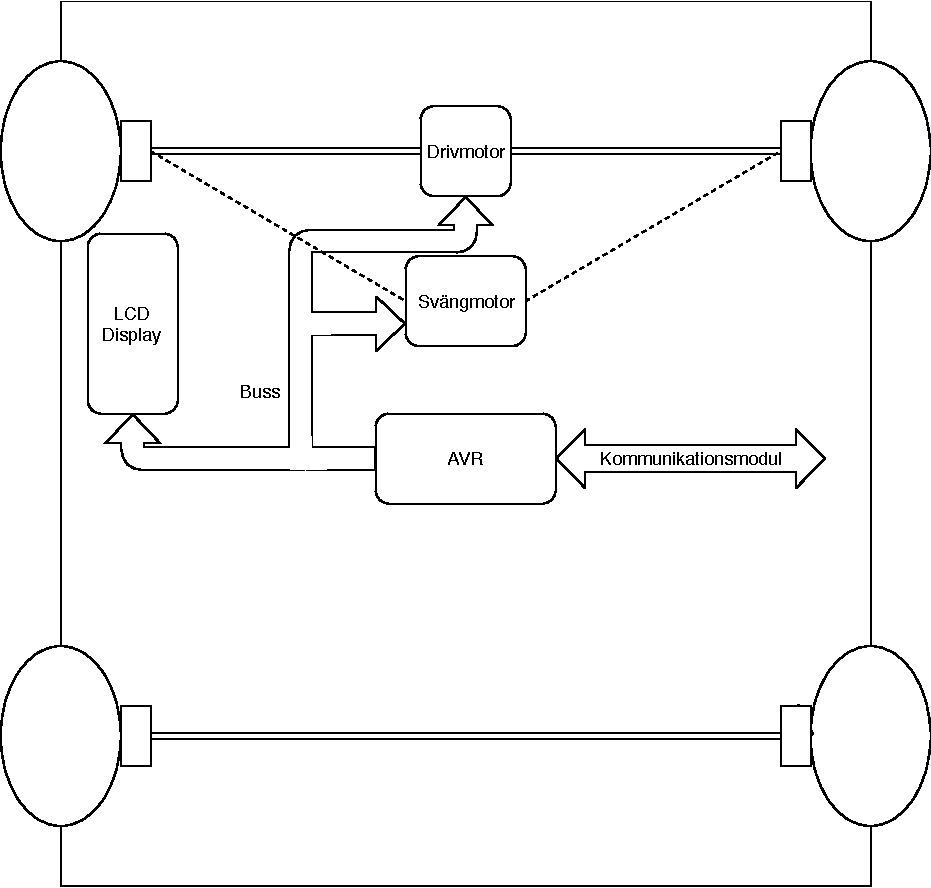
\includegraphics[width=0.6\linewidth]{kravspec/figures/styrmodul.pdf}
    \caption{Styrmodul}
    \label{fig:styrmodul}
\end{figure}

\subsection{Beskrivning}
Styrmodulen har som uppgift att ställa hjulen i rätt position samt att Taxin håller rätt hastighet. Styrmodulen är kopplad till kommunikationsmodulen ifrån den får information om hur Taxins hjul ska bete sig. Styrmodulen består av en kontroller, en drivmotor och en styrmotor. Styrmotorns uppgift är att hjulen ska vara i rätt position så att TAxin åker i önskad riktning. Drivmotorn är den motor som gör att bilen får en hastighet. Alltså köra fram eller bakåt.

\clearpage
\section{Sensormodul}
\subsection{Beskrivning}
Sensormodulen består av enhetens alla sensorer och en microprocessor. Dess
uppgift är att hantera information från de olika sensorerna och även
ut
\subsection{Gränssnitt}
\subsection{Krav}

\end{document}
